\section{Intégrale de \textsc{Dirichlet}}\label{sec:intDirichlet}

\todoinline{Peut-être pourrait on ajouter son utilisation en physique (un truc en diffration). Pour moi les souvenirs sont un peu lointains...}

\todoinline{Je mets dans les documents le fichier bestiaire.pdf qui appelle cette intégrale "intégrale de Cauchy" et qui donne plusieurs preuves abordables, la première avec lemme de Riemann-Lebesgue. On en choisit une ? deux ? Qu'en penses tu ?}

\todoarmand{J'aime bien l'exercice 167 avec cette idée de "perturber" l'intégrande avec $e^{-xt}$. Je trouve ça plus naturel que de supposer des relations non triviales ou introduire des fonctions sans comprendre d'où elles viennent. \\
On pourrait aussi ajouter le 170 qui peut être intéressant avec l'équation différentielle.}

\todoarmand{J'ajoute ces énoncés à la fin de la section}

\todoinline{Je commente ci-dessous ce que je pense des différentes parties}




\begin{prop}{}
    L'intégrale de \textsc{Dirichlet} (1829) est l'intégrale de la fonction sinus cardinal sur la demi-droite des réels positifs
    $$\int_{0}^{+\infty} \frac{\sin x}{x} \d x = \frac{\pi}{2}.$$
\end{prop}

\begin{marginfigure}[0cm]
    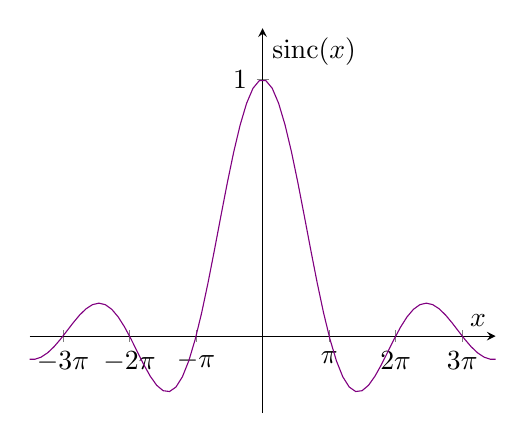
\begin{tikzpicture}
\begin{axis}[
    width=7.5cm,
    % grid=both,
    xmin=-11,
    xmax=11,
    ymin=-0.3,
    ymax=1.2,
    xlabel=$x$,
    ylabel=$\mathrm{sinc}(x)$,
    axis lines=center,
    xticklabels={$-3\pi$, $-2\pi$, $-\pi$, $\pi$, $2\pi$, $3\pi$},
    xtick={-3*3.141592, -2*3.141592, -3.141592, 3.141592, 2*3.141592, 3*3.141592},
    ytick={0, 1}
]
  \addplot[
    domain=-15:15,
    violet,
    ultra thick,
    samples=100,
  ] plot[thin] {sin(deg(x))/x};
\end{axis}
\end{tikzpicture}
\end{marginfigure}

\begin{preuve}
Une preuve utilisant le théorème des séries alternées.

\begin{enumerate}
\item La fonction $t \mapsto \frac{\sin t}{t}$ est continue sur $]0, 1]$. Comme elle est prolongeable par la valeur $1$ en $0$, elle est intégrable sur $]0, 1]$.

\item Soit $n \geq 1$.
\[
\int_{n\pi}^{(n+1)\pi} \frac{\sin t}{t} \d t = (-1)^n \int_0^\pi \frac{\sin u}{u + n \pi} \d u
\]
En notant $u_n$ cette quantité, comme sinus est positive sur $[0,\pi]$,
\begin{enumerate}
\item $u_n u_{n+1} \leq 0$,
\item $\abs{u_n} \leq \frac{1}{n\pi} \int_0^\pi \sin(u) \d u$ soit $u_n \to 0$,
\item $\abs{u_{n+1}} \leq \abs{u_n}$.
\end{enumerate}
Ainsi, d'après le théorème des séries alternées, $\sum u_n$ converge. Attention, la fonction $x \mapsto \int_0^x \frac{\sin t}{t} \d t$ n'est pas monotone et on ne peut donc pas encore conclure.

\item On pose $n_x = \left\lfloor\frac{x}{\pi}\right\rfloor$. En posant $F(x) = \int_1^{n_x\pi} \frac{\sin t}{t} \d t + \int_{n_x}^x \frac{\sin t}{t} \d t$, le premier terme converge d'après la question précédente. Le second est majoré par une quantité qui tend vers $0$.
\end{enumerate}
\end{preuve}

\begin{preuve}
Une preuve utilisant l'intégration par parties.
\begin{enumerate}
\item Les fonctions $u : t \mapsto -\cos(t)$ et $v : t \mapsto 1/t$ sont de classe $\mathscr{C}^1$ sur $[1,+\infty[$ et $\lim_{+\infty} u v = 0$. Ainsi, $\int_1^{+\infty} \frac{\sin t}{t} \d t$ et $\int_1^{+\infty} \frac{\cos(t)}{t^2}$ sont de même nature.
\begin{enumerate}
\item $t \mapsto \frac{\cos(t)}{t^2}$ est continue sur $[1,+\infty[$.
\item $\frac{\abs{\cos(t)}}{t^2} \leq \frac{1}{t^2}$ est intégrable sur $[1,+\infty[$.
\end{enumerate}
D'après les théorèmes de comparaison, $t \mapsto \frac{\abs{\cos(t)}}{t^2}$ est intégrable et $\int_1^{+\infty} \frac{\cos(t)}{t^2} \d t$ converge. Ainsi, $\int_1^{+\infty} \frac{\sin t}{t} \d t$ converge.
\end{enumerate}
\end{preuve}

\begin{remarque}
L'intégration par parties préserve la régularité de l'intégrale mais ne préserve pas l'intégrabilité.
\end{remarque}

\todoinline{Sous section "Régularité du sinus cardinal sur $\R$" déplacée dans la section "Prolongement de fonctions" mais toujours à voir si on la garde}

%-----------
\subsection{Non intégrabilité}

\begin{prop}{}
    La fonction sinus cardinal $\mathrm{sinc}:t \mapsto \frac{\sin(t)}{t}$ n'est pas intégrable sur $]0, +\infty[$.
\end{prop}

\begin{preuve}
    \marginnote[0cm]{Source : \href{https://www.agreg-maths.fr/uploads/versions/1175/dirichlet.pdf}{Intégrale de \textsc{Dirichlet} -- Florian \textsc{Dussap}}}
    Soit $N \in \Ne$, alors:
    \begin{align*}
        \int_0^{N \pi} \frac{|\sin x|}{x} \d x &= \sum_{k=0}^{N-1} \int_{k \pi}^{(k+1) \pi} \frac{|\sin x|}{x} \d x \\
        \text{par un changement de variable } &= \sum_{k=0}^{N-1} \int_0^\pi \frac{|\sin x|}{x + k \pi} \d x \\
        &\geqslant \sum_{k=0}^{N-1} \frac{1}{(k+1) \pi} \int_0^\pi \sin x \d x \\
        &\geqslant \frac{2}{\pi} \sum_{k=1}^N \frac{1}{k} \xrightarrow[N \to + \infty]{} + \infty.
    \end{align*}
\end{preuve}

%-----------        
\subsection{Calcul via le lemme de Lebesgue}

\begin{exercice}
\begin{enumerate}
    \item Calculer $I_n = \int_0^\pi \frac{\sin \left(n + \frac{1}{2}\right)t}{2 \sin \frac{t}{2}} \d t$. \\
    \emph{Indication :} Calculer $I_{n+1} - I_n$. 

    \item Montrer que la fonction définie sur $\interof{0}{\pi}$ par $f(x) = \frac{1}{x} - \frac{1}{2 \sin \frac{x}{2}}$ peut être prolongée à $\interff{0}{\pi}$ en une fonction de classe $\mathscr{C}^1$. 
    \item En déduire la valeur de l'intégrale $I = \int_0^{+\infty} \frac{\sin t}{t} \d t$.\\
    \emph{Indication :} On utilisera le lemme de Lebegue
\end{enumerate}
\end{exercice}

\begin{preuve}
\begin{enumerate}
\item En utilisant les formules de trigonométrie,
\begin{align*}
I_{n+1} - I_n
&= \int_0^\pi \frac{\sin\left(n + 1 + \frac{1}{2}\right) t - \sin\left(n + \frac{1}{2}\right) t}{2 \sin \frac{t}{2}} \d t\\
&= \int_0^\pi \cos (n + 1) t \d t
= \frac{1}{n + 1} \left[\sin(n + 1) t\right]_{0}^\pi
= 0.
\end{align*}

Ainsi, la suite $(I_n)$ est constante et $I_0 = \frac{\pi}{2}$. Donc, pour tout $n$ entier naturel, $I_n = \frac{\pi}{2}$.

\item La fonction $f$ est continue et dérivable sur $]0; \pi]$. De plus, pour tout réel $x \in ]0; \pi]$,
$f(x) = \frac{2 \sin(x/2) - x}{2 x \sin(x/2)}$.

En utilisant les développements limités classiques,
\[
f(x)
\sim -\frac{\frac{x^3}{24}}{x^2}
\sim -\frac{x}{24}.
\]
Ainsi, $f$ est prolongeable par continuité en $0$ par $f(0) = 0$.

\medskip

La fonction $f$ est dérivable sur $]0;\pi]$ et pour tout $x \in ]0;\pi]$,
\begin{align*}
f'(x)
&= -\frac{1}{x^2} + \frac{\cos(x/2)}{4 \sin(x/2)^2}\\
&= \frac{\cos(x/2) - 4 \sin(x/2)^2}{4 x^2 \sin(x/2)^2}\\
&\sim -\frac{1}{24}.
\end{align*}

Ainsi, $\lim_{x\to0} f'(x) = -\frac{1}{24}$. D'après le théorème de prolongement dérivable, la fonction $f$ est prolongeable en une fonction de classe $\mathscr{C}^1$ sur $[0; \pi]$.

\item En utilisant le lemme de Lebesgue pour les fonctions de classe $\mathscr{C}^1$, on en déduit que
\begin{align*}
\int_0^{(n + 1/2) \pi} \frac{\sin t}{t} \d t
&= \int_0^\pi \frac{\sin (n + 1/2) t}{t} \d t\\
&= \int_0^\pi \left[ \frac{\sin(n + 1/2) t}{t} - \frac{\sin (n + 1/2) t}{2 \sin (t/2)} + \frac{\sin (n + 1/2) t}{2 \sin(t/2)} \right] \d t\\
&= \int_0^\pi f(t) \sin((n + 1/2) t) \d t - I_n.
\end{align*}
Comme $f$ est de classe $\mathscr{C}^1$, d'après le lemme de Lebesgue,
\[
\lim_{n\to+\infty} \int_0^\pi f(t) \sin((n + 1/2) t) \d t = 0.
\]

Finalement, $I = \frac{\pi}{2}$.
\end{enumerate}
\end{preuve}

%-----------
\subsection{Calcul via une intégrale à paramètre}

\begin{comment}
\begin{exercice}
    Exercice 167 p.179 (bestiaire.pdf) \\
    On considère l'application $f(x) = \int_0^\infty \frac{\sin(t)}{t} \e^{-xt} \d t$.
    \begin{enumerate}
        \item Montrer que $f \in \mathscr{C}^1(\Rpe)$.
        \item En déduire une forme explicite de $f$ sur $\Rpe$. 
        \item Montrer que $f$ est continue à l'origine. 
        \item En déduire que $\int_0^\infty \frac{\sin(t)}{t} \d t = \frac{\pi }{2}$.
    \end{enumerate}
\end{exercice}
\end{comment}

\begin{comment}
\begin{exercice}
Soit la transformée de \textsc{Laplace} de la fonction sinus cardinal:
$$F:x \to \int_{0}^{+ \infty} \exp(-xt) \frac{\sin (t)}{t} \d t$$
    
\begin{enumerate}
    \item \emph{Montrer que $F$ est définie sur $\Rp$.}
    \item \emph{Calculer $F$ sur $\Rpe$, en déduire la valeur de la fonction de \textsc{Dirichlet}}
\end{enumerate}
\end{exercice}
\begin{preuve}
\begin{enumerate}
\item Montrons que $F$ est bien définie. D'une part, $\lim_{t \to 0} \exp(-x t) \frac{\sin t}{t} = 1$ donc l'intégrande est prolongeable par continuité en $0$ et est donc intégrable sur $]0, 1]$.
\begin{enumerate}
        \item Si $x > 0$, majorer l'intégrande par $t \mapsto \exp(-xt)$.
        \item Si $x = 0$, montrer le prolongement par continuité de la fonction sinus cardinal en $0$ puis intégrer la fonction sinus cardinal par parties sur $[1, +\infty]$.
    \end{enumerate}
\end{enumerate}
\end{preuve}
\end{comment}

%---------------

\begin{exercice}%
{RMS - Autres Écoles - 178}%
{IMT}%
{16}%
On note $I = \int_0^{+\infty} \frac{\sin(t)}{t} \d t$ et $F(x) = \int_0^{+\infty} \frac{\sin(t)}{t} (1 - \e^{-x t}) \d t$.
\begin{enumerate}
\item Montrer que $I$ est bien définie.
\item Montrer que $F$ est définie sur $[0,+\infty[$, que $F$ est continue sur $[0, +\infty[$ et que $F$ est dérivable sur $]0, +\infty[$.
\item En déduire la valeur de $I$.
\end{enumerate}
\end{exercice}

\begin{preuve}
\begin{enumerate}
\item Les fonctions $u : t \mapsto 1 - \cos(t)$ et $v : t \mapsto \frac{1}{t}$ sont de classe $\mathscr{C}^1$ sur $\R_+^*$. De plus, le produit $u v$ a des limites nulles en $0$ et $+\infty$. Ainsi, d'après la formule d'intégration par parties, $I$ a même nature que
\[
\int_0^{+\infty} \frac{1 - \cos t}{t^2} \d t,
\]
dont l'intégrande est continue sur $]0, +\infty[$, prolongeable par continuité par $\frac{1}{2}$ en $0$ et majorée par $t \mapsto \frac{1}{t^2}$ en $+\infty$, donc est intégrable.

\item 
\begin{enumerate}
\item $F(x)$ est la somme de $I$ et de l'intégrale de $f : (x, t) \mapsto \frac{\sin t}{t} \e^{- x t}$.
\begin{enumerate}
\item $f(x, .)$ est continue sur $\R_+^*$.
\item $f(x, .)$ admet pour limite $1$ en $0$.
\item $\abs{f(x, .)}$ est un $o(1/t^2)$ en $+\infty$.
\end{enumerate}
Ainsi, $F$ est bien définie sur $\R_+$.

\item Pour la continuité, on ne peut pas espérer appliquer le théorème de convergence dominée directement car $t \mapsto \frac{\sin t}{t}$ n'est pas intégrable. On utilise donc une intégration par parties en considérant $u : t \mapsto \int_t^{+\infty} \frac{\sin t}{t} \d t$ et $v : t \mapsto (1 - \e^{-x t})$. Comme le produit $u v$ admet des limites nulles en $0$ et $+\infty$, alors
\begin{align*}
F(x) &= -x \int_{0}^{+\infty} u(t) \e^{- x t} \d t \\
&= -\int_0^{+\infty} u\left(\frac{v}{x}\right) \e^{-v} \d v.
\end{align*}
Comme $u$ possède des limites en $0$ et $+\infty$, elle est bornée sur $\R_+$ et
\[
\abs{u\left(\frac{u}{x}\right) \e^{-u}} \leq M \e^{-u},
\]
qui est une fonction intégrable. Ainsi, d'après le théorème de convergence dominée,
\[
\lim_{x\to0} F(x) = -\int_0^{+\infty} \lim_{t\to+\infty} u(t) \e^{-v} \d v = 0.
\]
Ainsi, $F$ est continue en $0$.

\item Avec les notations de la question précédente,
\[
\forall\, x \in [a, +\infty[,\, \abs{\frac{\partial f}{\partial x}(x, t)} \leq \e^{-a t}.
\]
Ainsi, la fonction $F$ est de classe $\mathscr{C}^1$ sur $[a, +\infty[$, donc sur $\R_+^*$.
\end{enumerate}

De plus, pour tout $x > 0$,
\[
F'(x) = \int_0^{+\infty} \sin(t) \e^{-x t} \d t = \frac{1}{1 + x^2}.
\]

\item D'après la question précédente, il existe une constante $C \in \R$ telle que
\[
\forall\, x > 0,\, F(x) = C + \arctan(x).
\]

Comme $F(0) = 0$, et par continuité de la fonction $F$, alors $C = 0$.

Enfin, $F(x) = I - \int_0^{+\infty} \frac{\sin t}{t} \e^{-x t} \d t$ et
\[
\abs{\int_0^{+\infty} \frac{\sin t}{t} \e^{-x t} \d t} \leq \int_0^{+\infty} \e^{-x t} \d t \leq \frac{1}{x}.
\]
Ainsi, $\lim_{x\to+\infty} F(x) = I$ et
\[
I = \frac{\pi}{2}.
\]
\end{enumerate}
\end{preuve}

%-----------
\subsection{Une preuve par équations différentielles}

\begin{exercice}
    Exercice 170 p. 184 \\
    Soient $f(x) = \int_0^\infty \frac{\sin(t)}{t+x} \d t$, $g(x) = \int_0^\infty \frac{\e^{-xt}}{t^2 + 1} \d t$. 
    \begin{enumerate}
        \item Montrer que $f, g \in \mathscr{C}^2(\Re)$. \\
        \textit{Pour $f$, on pourra commencer par montrer que $f(x) = \int_0^\infty \frac{1 - \cos(t)}{(t+x)^2} \d t$.}
        \item Montrer que $f$ et $g$ sont solutions de l'équation différentielle $y'' + y = \frac{1}{x}$.

        \item En déduire que $f-g$ est $2 \pi$-périodique (sur son domaine de définition).

        \item Montrer que $f$ et $g$ tendent vers $0$ en $+\infty$, puis que $f = g$.
        \item En déduire la valeur de $\int_0^\infty \frac{\sin(t)}{t} \d t$.
    \end{enumerate}
\end{exercice}

\begin{preuve}
\begin{enumerate}
\item On pose $g : (x, t) \mapsto \frac{\e^{-x y}}{t^2 + 1}$. Alors, pour tout $(x, t) \in [a, +\infty[ \times \R_+$,
\begin{align*}
\abs{g(x, t)} &\leq \frac{1}{1 + t^2},\\
\abs{\frac{\partial g}{\partial x}(x, t)} &\leq \frac{t \e^{-a t}}{1 + t^2},\\
\abs{\frac{\partial^2 g}{\partial x^2}(x, t)} &\leq \frac{t^2 \e^{-a t}}{1 + t^2}.
\end{align*}

Ainsi, d'après le théorème de dérivation sous le signe intégral, la fonction $g$ est de classe $\mathscr{C}^2$ sur $\R_+^*$ et
\begin{align*}
g''(x)
&= \int_0^{+\infty} \frac{t^2 \e^{-x t}}{1 + t^2} \d t\\
&= \int_0^{+\infty} \frac{(1 + t^2 - 1) \e^{-x t}}{1 + t^2} \d t\\
&= \int_0^{+\infty} \e^{-x t} \d t - g(x)\\
&= \frac{1}{x} - g(x).
\end{align*}

\item En utilisant l'intégration par parties vue au début du chapitre,
\begin{align*}
f(x)
&= \left[\frac{1 - \cos(t)}{t + x}\right]_0^{+\infty} + \int_0^{+\infty} \frac{1 - \cos(t)}{(t + x)^2} \d t\\
&= \int_0^{+\infty} \frac{1 - \cos(t)}{(t + x)^2} \d t.
\end{align*}
En posant $h(x, y) = \frac{1 - \cos(t)}{(t + x)^2}$, pour tout $(x, t) \in [a, +\infty[ \times \R_+$,
\begin{align*}
\abs{h(x, t)} &\leq \frac{1}{(t + a)^2}\\
\abs{\frac{\partial h}{\partial x}(x, t)} &\leq \frac{2}{(t + a)^3}\\
\abs{\frac{\partial^2 h}{\partial x^2}(x, t)} &\leq \frac{6}{(t + a)^3}.
\end{align*}
Ainsi, la fonction $f$ est de classe $\mathscr{C}^2$ sur $\R_+^*$ et, à l'aide d'intégrations par parties,
\begin{align*}
f''(x)
&= \int_0^{+\infty} \frac{6 (1 - \cos(t))}{(t + x)^4} \d t\\
&= \int_0^{+\infty} \frac{2 \sin(t)}{(t + x)^3} \d t\\
&= \int_0^{+\infty} \frac{\cos(t)}{(t + x)^2} \d t\\
&= \int_0^{+\infty} \frac{\d t}{(t + x)^2} - \int_0^{+\infty} \frac{1 - \cos t}{(t + x)^2} \d t\\
&= \frac{1}{x} - f(x).
\end{align*}

\item Comme $f - g$ est solution de l'équation différentielle $y'' - y = 0$, alors $f - g$ est $2\pi$-périodique.

\item En utilisant l'expression précédente,
\begin{align*}
f(x)
&= \frac{1}{x} - \int_0^{+\infty} \frac{2 \sin(t)}{(t + x)^3} \d t.
\end{align*}
Or, $\abs{\int_0^{+\infty} \frac{2 \sin(t)}{(t + x)^3} \d t} \leq \frac{2}{x^2}$. Ainsi, $f(x) \sim_{+\infty} \frac{1}{x}$.

De même, en $+\infty$,
\begin{align*}
\abs{g(x)}
&\leq \int_0^{+\infty} \e^{- x t} \d t
\leq \frac{1}{x}.
\end{align*}

D'après les points précédents, $\lim_{x\to+\infty} (f - g) = 0$. Comme $f - g$ est périodique, alors $f - g$ est la fonction nulle.

Ainsi,
\[
\forall\, x > 0,\, \int_0^{+\infty} \frac{\sin(t)}{t + x} \d t = \int_0^{+\infty} \frac{\e^{-x t}}{t^2 + 1} \d t.
\]

\item Comme $\abs{\frac{\e^{-x t}}{t^2 + 1}} \leq \frac{1}{1 + t^2}$, d'après le théorème de convergence dominée,
\[
\lim_{x\to 0} \int_0^{+\infty} \frac{\e^{-x t}}{t^2 + 1} \d t
= \int_0^{+\infty} \frac{\d t}{1 + t^2}
= \frac{\pi}{2}.
\]

De plus,
\begin{align*}
\abs{\int_0^{+\infty} \frac{\sin(t)}{t + x} \d t - \int_0^{+\infty} \frac{\sin(t)}{t} \d t}
\leq \int_0^1 \frac{x \abs{\sin(t)}}{t (t + x)} \d t + \int_1^{+\infty} \frac{x \abs{\sin t}}{t (t + x)} \d t.
\end{align*}

Le premier terme tend vers $0$ par convergence dominée, avec la domination $t \mapsto \frac{\abs{\sin t}}{t}$ qui est bien intégrable sur $[0, 1]$.

Le second terme tend vers $0$ par domination par $x \int_1^{+\infty} \frac{\d t}{t^2}$.

Finalement, on obtient
\[
\int_0^{+\infty} \frac{\sin t}{t} \d t
= \int_0^{+\infty} \frac{1}{1 + t^2} \d t
= \frac{\pi}{2}.
\]
\end{enumerate}
\end{preuve}


%-----------
\subsection{Pour aller plus loin}

\todoinline{On pourrait garder cette ouverture en citant ENSAIT-MP-1996 comme source. On peut également ouvrir vers les intégrales de Borwein}

\todoarmand{J'aime bien l'idée de l'ouverture vers les intégrales de Borwein. C'est aussi l'occasion d'évoquer la transformée de Fourier et le produit de convolution il me semble, mais c'est peut être trop ambitieux. Une ressource intéressante \url{https://perso.telecom-paristech.fr/rioul/publis/202301rioul.pdf}}

À l'aide d'intégrations par parties, on peut montrer que
\[
\int_0^{+\infty} \left(\frac{\sin t}{t}\right)^2 \d t
= \int_0^{+\infty} \left(\frac{\sin t}{t}\right)^4 \d t
= \frac{\pi}{2}.
\]

En utilisant la linéarisation du sinus, on peut montrer que
\[
\int_0^{+\infty} \frac{(\sin t)^3}{t^2} \d t = \frac{3 \ln(3)}{4}.
\]